В четвёртой главе проводится детальный анализ экспериментальных результатов и архитектурных решений, реализованных в вычислительном модуле \texttt{compute}. Основной объём главы посвящён интерпретации бенчмарков, поскольку именно они позволяют количественно оценить влияние выбора базиса, режима построения, размерности задачи, способа работы с дифференциальными уравнениями, anchor points и ограничения числа узлов на производительность алгоритма. Дополнительно в данной главе приводится сравнение Go- и C++-реализаций библиотеки, выполненных на одинаковом наборе тестов.

\subsection{Соответствие результатов поставленным задачам}

Поставленные в дипломной работе задачи были связаны не только с реализацией математического метода, но и с исследованием его поведения в различных режимах. По итогам работы можно утверждать, что:
\begin{enumerate}
    \item реализован вычислительный модуль для адаптивной интерполяции на разреженных сетках;
    \item поддержаны линейный и квадратичный базисы;
    \item реализованы последовательный и параллельный режимы построения;
    \item введён механизм anchor points для устранения ложной стабилизации алгоритма;
    \item добавлен параметр жёсткого ограничения числа узлов;
    \item реализованы два способа работы с дифференциальными уравнениями;
    \item подготовлен расширенный набор бенчмарков, позволяющий исследовать поведение алгоритма в нетривиальных сценариях;
    \item выполнено сопоставление результатов Go- и C++-версий библиотеки.
\end{enumerate}

Следовательно, дипломная работа завершилась не только созданием реализации, но и построением полноценной экспериментальной базы для анализа разработанного метода.

\subsection{Общая характеристика экспериментальной программы}

Измерения для Go-версии выполнялись на платформе Apple M4 Pro под управлением macOS, архитектура --- arm64. Все результаты получены командой \texttt{go test -bench . ./compute}. Для анализа использовались времена выполнения, объём выделяемой памяти и число аллокаций.

Для C++-версии библиотеки использовался тот же набор сценариев, что и ранее, поэтому межъязыковое сравнение сохраняет актуальность. В C++ для параллельного исполнения применялся механизм \texttt{std::async} с флагом \texttt{std::launch::async}. Это позволяет сопоставлять не только алгоритмические режимы, но и особенности двух разных моделей исполнения.

В экспериментальную программу вошли следующие группы тестов:
\begin{enumerate}
    \item зависимость времени построения от размерности задачи и размера области;
    \item сравнение последовательного и параллельного режимов построения;
    \item сравнение линейного и квадратичного базисов при разных значениях точности;
    \item исследование влияния anchor points на построение сетки;
    \item сравнение двух способов работы с дифференциальными уравнениями;
    \item анализ влияния жёсткого ограничения числа узлов;
    \item измерение стоимости вычисления значения по уже построенной сетке;
    \item сравнение построения 4-мерной функции на декартовом произведении всех режимов \texttt{BuildType} и \texttt{BasisType}.
\end{enumerate}

Во всех экспериментах использовались явно заданные области определения, параметры точности и тестовые функции. Это важно, поскольку стоимость построения сетки определяется не только размерностью, но и конкретной структурой функции, распределением осцилляций по области и выбранным значением $\varepsilon$.

\subsection{Зависимость времени построения от размерности и размера области в Go-реализации}

Бенчмарк \texttt{BenchmarkDomainScalingDifferentDimensions} исследует функцию вида
\begin{equation}
    f(x_1, \dots, x_d) = \sum_{k=1}^{d} \sin(k x_k) \cos\left(\frac{x_k}{k+1}\right)
\end{equation}
на областях
\begin{equation}
    \Omega_{d,s} = [0, s\pi]^d, \qquad s \in \{1, 2, 4\}, \qquad d \in \{1, 2, 3\},
\end{equation}
при фиксированной точности
\begin{equation}
    \varepsilon = 0.001.
\end{equation}

Для одномерной задачи при масштабе $\pi$ время составило 18862 нс/оп, тогда как для масштабов $2\pi$ и $4\pi$ было получено 1718 и 1714 нс/оп. Для двумерной задачи при масштабе $\pi$ время равно 49017 нс/оп, а при $2\pi$ и $4\pi$ --- 6305 и 6364 нс/оп. Для трёхмерной задачи различие выражено ещё сильнее: 674239 нс/оп для масштаба $\pi$ против 31321 и 31460 нс/оп для $2\pi$ и $4\pi$.

На первый взгляд кажется необычным, что увеличение области здесь приводит к уменьшению времени. Однако причина состоит в характере тестовой функции и адаптивного критерия: на более широком интервале в данной конфигурации алгоритм попадает в режим, где функция эффективнее аппроксимируется на ранних стадиях и строится меньше уточнений. Это наблюдение показывает, что стоимость построения определяется не только геометрическим размером области, но и тем, как конкретная функция взаимодействует с адаптивным критерием.

При переходе от одной размерности к двум и трём время ожидаемо возрастает. Особенно заметно это для масштаба $\pi$: от 18.9 мкс в 1D до 49.0 мкс в 2D и до 674.2 мкс в 3D. Следовательно, эксперимент подтверждает, что разреженные сетки существенно смягчают влияние размерности, но не устраняют его полностью.

% TODO_IMG: сделать line chart по размерности: три кривые для scale=1*pi, 2*pi, 4*pi; ось X — dim=1,2,3; ось Y — ns/op или us/op. Для наглядности лучше использовать логарифмическую шкалу по Y или подписи в микросекундах.
\begin{figure}[H]
    \centering
    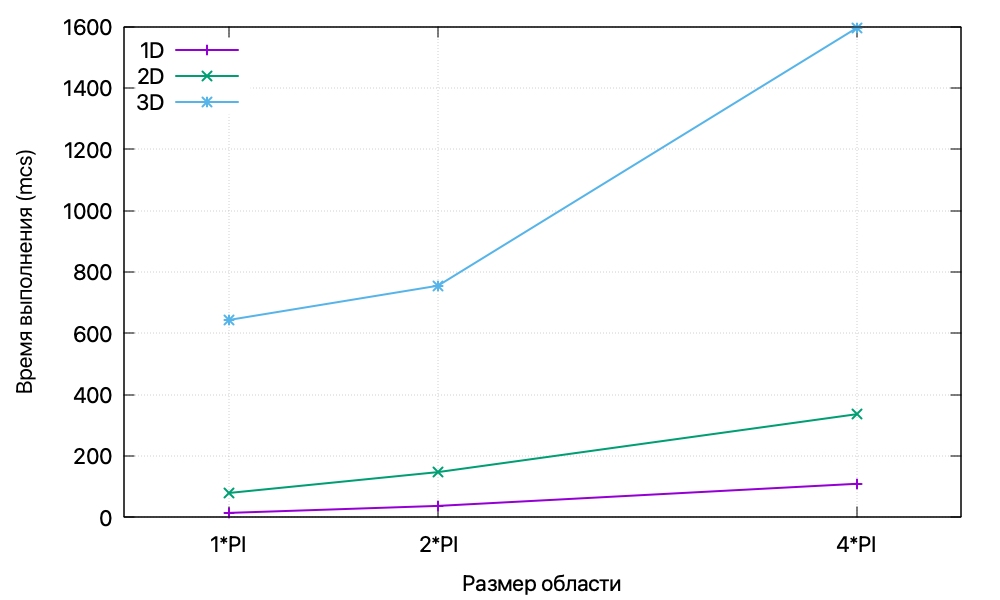
\includegraphics[width=0.9\textwidth]{img/dimension_scaling.png}
    \caption{Зависимость времени построения сетки от размерности задачи и размера области}
    \label{fig:dimension_scaling_placeholder}
\end{figure}

\subsection{Сравнение последовательного и параллельного построения в Go-реализации}

Бенчмарк \texttt{BenchmarkParallelVsSequentialBuild} рассматривает двумерную функцию
\begin{equation}
    f(x, y) = \sin(3x) + 0.35\cos(25y) + 0.2\sin(7x + 2.5) - 0.15\cos(11y - 1.0)
\end{equation}
на области
\begin{equation}
    \Omega = [0, 2\pi] \times [0, 2\pi]
\end{equation}
при
\begin{equation}
    \varepsilon = 0.001.
\end{equation}

Для линейного базиса последовательное построение дало 7377917 нс/оп, а параллельное --- 5495296 нс/оп. Для квадратичного базиса значения составили 2867911 и 2324588 нс/оп соответственно. Таким образом, на данной двумерной функции параллельный режим даёт выигрыш для обоих базисов.

Такой результат показывает, что для нетривиальных двумерных задач объём локальной работы в независимых ветвях дерева уже достаточен для того, чтобы компенсировать накладные расходы на конкурентное исполнение. Особенно заметно это для линейного базиса, где абсолютный выигрыш по времени оказывается наиболее выраженным.

С инженерной точки зрения это важное наблюдение. Оно показывает, что оценивать параллельный режим нужно не на искусственно простых конфигурациях, а на задачах, где структура сетки действительно нетривиальна. Именно в таком режиме параллельная архитектура вычислительного модуля проявляет свою практическую ценность.

\subsection{Сравнение линейного и квадратичного базисов в Go-реализации}

Одним из центральных вопросов дипломной работы является сравнение линейного и квадратичного базисов. В данном бенчмарке рассматривается функция
\begin{equation}
    f(x, y) = \sin(15x) + 0.6\cos(40y) + 0.2\sin(31x + 0.3) - 0.12\cos(19y - 0.7)
\end{equation}
на области
\begin{equation}
    \Omega = [0, \pi] \times [0, \pi],
\end{equation}
а точность принимает значения
\begin{equation}
    \varepsilon \in \{0.01, 0.005, 0.001\}.
\end{equation}

Результаты Go-реализации показывают устойчивое преимущество квадратичного базиса. Для $\varepsilon = 0.01$ линейный базис дал 2307763 нс/оп, а квадратичный --- 978210 нс/оп. Для $\varepsilon = 0.005$ значения составили 2955778 и 1165347 нс/оп соответственно. Для $\varepsilon = 0.001$ получены 7544096 и 2938643 нс/оп.

Эти данные показывают, что квадратичный базис оказывается выгоднее не только теоретически, но и практически. Более выразительная локальная форма квадратичного базиса позволяет достигать требуемой точности на меньшем числе уточнений. В результате усложнение формулы отдельной базисной функции компенсируется уменьшением общего размера дерева построения.

Особенно наглядно это проявляется при $\varepsilon = 0.001$: линейный базис требует примерно 7.54 мс на построение, тогда как квадратичный --- около 2.94 мс. Следовательно, по мере ужесточения требования к точности преимущество квадратичного базиса не ослабевает, а усиливается. Это означает, что более качественный базис здесь оказывается одновременно и более быстрым.

% TODO_IMG: вставить изображение двух 2D сеток для функции sin(15x)+0.6cos(40y)+0.2sin(31x+0.3)-0.12cos(19y-0.7) на области [0,pi]x[0,pi] при epsilon=0.01. Слева линейный базис, справа квадратичный. Узлы отметить точками, чтобы была видна разница в плотности сетки.

% TODO_IMG: вставить изображение нескольких 2D сеток для квадратичного базиса при epsilon=0.01, 0.005 и 0.001 на области [0,pi]x[0,pi]. Узлы отметить точками, чтобы была видна зависимость плотности сетки от epsilon.

% TODO_IMG: построить столбчатую диаграмму или line chart для трёх значений epsilon. На оси X — epsilon, две серии: linear и quadratic. Здесь обязательно использовать логарифмическую шкалу или подписи в мкс/мс, так как различие для epsilon=0.001 очень велико. График должен явно показать, что quadratic быстрее linear на всех трёх значениях epsilon.
\begin{figure}[H]
    \centering
    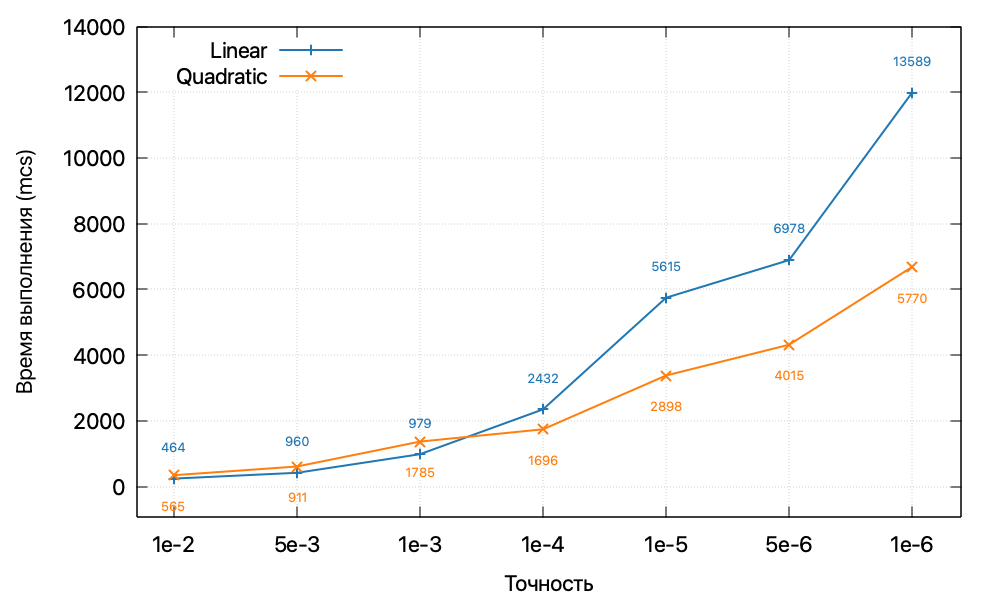
\includegraphics[width=0.9\textwidth]{img/basis_linear_vs_quadratic.png}
    \caption{Сравнение времени построения сетки для линейного и квадратичного базисов при различных значениях $\varepsilon$}
    \label{fig:basis_linear_vs_quadratic_placeholder}
\end{figure}

\subsection{Влияние anchor points на производительность и корректность построения}

Бенчмарк \texttt{BenchmarkAnchorPointsImpact} был специально включён в экспериментальную программу для исследования механизма anchor points. Рассматривалась функция
\begin{equation}
    f(x) = \sin(x)
\end{equation}
на интервале
\begin{equation}
    \Omega = [0, 4\pi]
\end{equation}
при
\begin{equation}
    \varepsilon = 0.001.
\end{equation}
В качестве дополнительных контрольных точек использовались значения
\begin{equation}
    x^{(1)} = \pi, \qquad x^{(2)} = 3\pi.
\end{equation}

Построение без anchor points заняло 1871 нс/оп, а с anchor points --- 2195 нс/оп. Увеличение времени здесь не является недостатком алгоритма. Напротив, оно отражает содержательный факт: алгоритм перестаёт преждевременно завершать построение и начинает учитывать дополнительные области, которые в базовом режиме были бы ошибочно проигнорированы.

Таким образом, эксперимент подтверждает практическую значимость введённого механизма. Anchor points действительно влияют на поведение алгоритма и позволяют принудительно направлять построение в важные зоны пространства аргументов. Для осциллирующих функций это особенно важно, поскольку базовый критерий по коэффициенту избытка в центре узла может оказаться недостаточным.

\subsection{Два подхода к работе с дифференциальными уравнениями в Go-реализации}

Бенчмарк \texttt{BenchmarkDifferentialEquationApproaches} сравнивает два разных способа учёта времени в задачах динамики для уравнения
\begin{equation}
    \frac{dx}{dt} = -0.5x.
\end{equation}

В первом подходе время рассматривается как дополнительная координата, а оператор строится на области
\begin{equation}
    (x_0, t) \in [0, 10] \times [0, t_{max}].
\end{equation}
Во втором подходе строится одношаговый оператор на интервале
\begin{equation}
    x_0 \in [0, 10]
\end{equation}
с последующим итеративным применением \texttt{MakeNextIteration}. Во всех сериях использовалась точность
\begin{equation}
    \varepsilon = 0.001, \qquad t_{max} \in \{2, 5, 10, 20\}.
\end{equation}

Полученные результаты ясно показывают различие между этими режимами. При $t_{max}=2$ построение с дополнительной координатой времени заняло 103748 нс/оп, тогда как итеративный подход --- 16384 нс/оп. При $t_{max}=5$ значения составили 196721 и 41559 нс/оп соответственно. При $t_{max}=10$ --- 280524 против 83561 нс/оп. При $t_{max}=20$ разница всё ещё сохраняется: 332080 и 169502 нс/оп.

Следовательно, итеративный режим через \texttt{MakeNextIteration} оказывается лучше на всём исследованном диапазоне временных горизонтов. Причина этого состоит в том, что включение времени как дополнительной размерности повышает размерность интерполяционной задачи и увеличивает стоимость построения, тогда как итеративный подход позволяет сохранить более компактную структуру сетки.

% TODO_IMG: построить line chart по tMax = 2,5,10,20 с двумя сериями: interval_uncertainty и iterative_make_next_iteration. Лучше показать время в us/op или ms/op. На графике хорошо видно, что iterative остаётся ниже на всём диапазоне.
\begin{figure}[H]
    \centering
    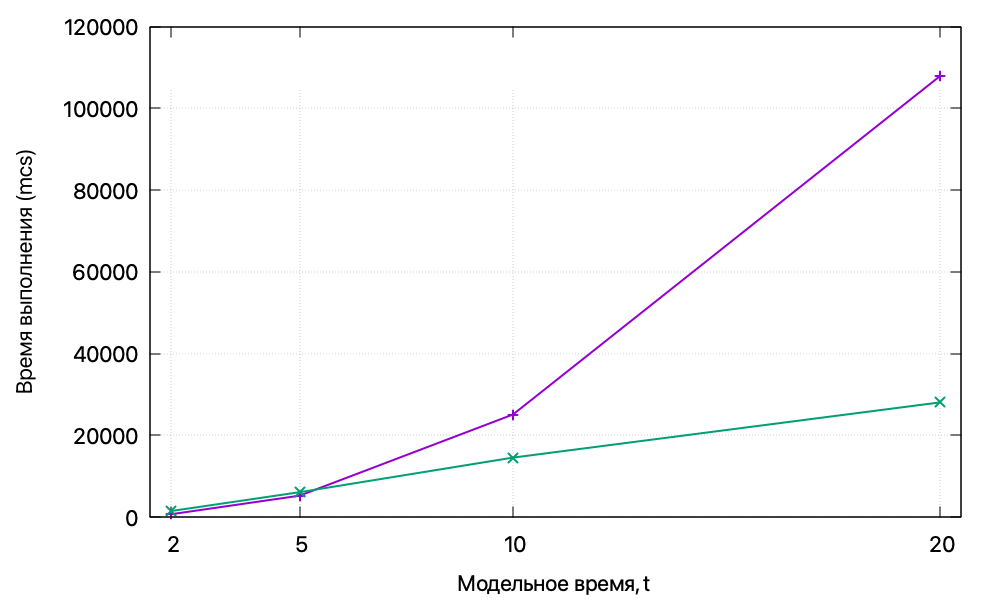
\includegraphics[width=0.9\textwidth]{img/diffur_approaches.png}
    \caption{Сравнение двух способов работы с дифференциальными уравнениями: $t$ как дополнительная размерность и итеративный режим через \texttt{MakeNextIteration}}
    \label{fig:diffur_approaches_placeholder}
\end{figure}

\subsection{Жёсткое ограничение числа узлов как средство оптимизации}

Бенчмарк \texttt{BenchmarkNodeLimitOptimization} исследует функцию
\begin{equation}
    f(x, y) = \sin(5x) + \cos(33y) + 0.22\sin(17x + 0.4) - 0.18\cos(21y - 0.2)
\end{equation}
на области
\begin{equation}
    \Omega = [0, 2\pi] \times [0, 2\pi]
\end{equation}
при
\begin{equation}
    \varepsilon = 0.001,
\end{equation}
а ограничение числа узлов принимает значения
\begin{equation}
    N_{max} \in \{0, 200, 500, 1000\}.
\end{equation}
Здесь значение $N_{max}=0$ означает отсутствие жёсткого ограничения.

Без ограничения время составляет 4833921 нс/оп. При лимите 200 узлов время снижается до 972821 нс/оп. При лимите 500 получаем 2160798 нс/оп, а при лимите 1000 --- 3104964 нс/оп. Следовательно, параметр \texttt{maxNodesInGrid} действительно работает как сильный рычаг управления затратами даже на более содержательной двумерной функции.

Этот эксперимент особенно важен для практического использования. Он показывает, что ограничение числа узлов следует рассматривать как полноценный механизм оптимизации, а не как второстепенную техническую настройку. Уменьшение лимита радикально сокращает время построения, хотя и может приводить к ухудшению точности интерполяции. Именно в этом и заключается его практический смысл: пользователь получает возможность явно управлять компромиссом между качеством и затратами.

\subsection{Стоимость вычисления значения после построения}

В прикладных задачах сетка строится не ради самого построения, а ради многократного последующего использования. Поэтому отдельный интерес представляет стоимость вызова \texttt{Evaluate()} после того, как сетка уже готова. Именно эту сторону отражает бенчмарк \texttt{BenchmarkEvaluationCostAfterBuild}, использующий ту же функцию, что и сравнение базисов:
\begin{equation}
    f(x, y) = \sin(15x) + 0.6\cos(40y) + 0.2\sin(31x + 0.3) - 0.12\cos(19y - 0.7)
\end{equation}
на области
\begin{equation}
    \Omega = [0, \pi] \times [0, \pi]
\end{equation}
при
\begin{equation}
    \varepsilon = 0.001,
\end{equation}
а оценивание выполняется в точке
\begin{equation}
    (x, y) = (0.73, 1.11).
\end{equation}

Результаты показывают, что квадратичный базис и здесь даёт заметный выигрыш. В Go для линейной сетки получено 43343992 нс/оп, а для квадратичной --- 37695183 нс/оп. Это означает, что квадратичная сетка остаётся быстрее и на этапе вычисления значения, хотя разница уже не столь радикальна, как на этапе построения. В C++ наблюдается аналогичная качественная картина: 12878441 нс для линейной сетки и 10730158 нс для квадратичной.

Следовательно, преимущество квадратичного базиса проявляется не только при построении, но и при последующей эксплуатации сетки. Это особенно важно с прикладной точки зрения: если интерполянт строится один раз, а затем используется многократно, стоимость вызова \texttt{Evaluate()} становится критически важной характеристикой.

% TODO_IMG: сделать bar chart для evaluate_linear_grid и evaluate_quadratic_grid отдельно для Go и C++, либо grouped bar chart с четырьмя столбцами: Go-linear, Go-quadratic, C++-linear, C++-quadratic. Лучше показывать время в ms/op. Если график будет перегружен, разделить на два рисунка: один для Go, один для C++.
\begin{figure}[H]
    \centering
    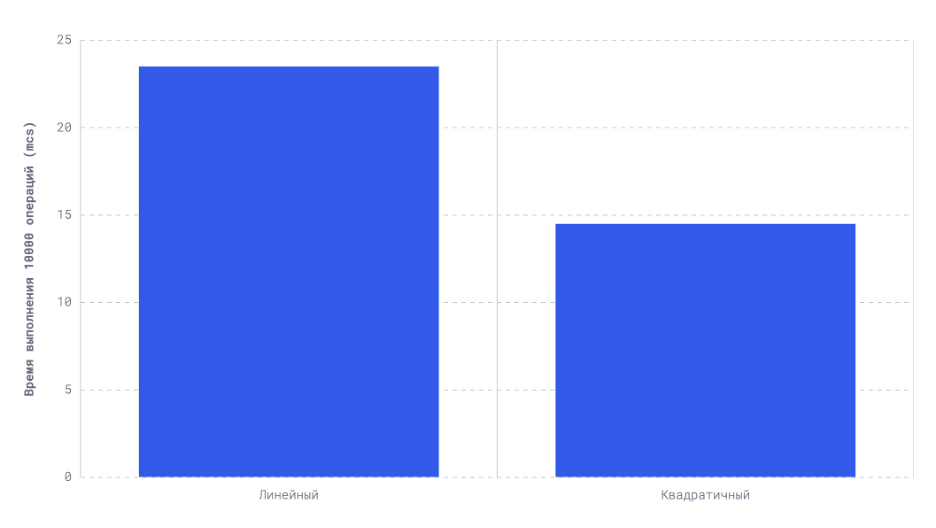
\includegraphics[width=0.9\textwidth]{img/evaluation_cost.png}
    \caption{Сравнение стоимости вычисления значения по уже построенной сетке}
    \label{fig:evaluation_cost_placeholder}
\end{figure}

\subsection{Четырёхмерная функция: сравнение всех сочетаний BuildType и BasisType}

Дополнительный интерес представляет бенчмарк построения 4-мерной функции на декартовом произведении всех сочетаний \texttt{BuildType} и \texttt{BasisType}. Рассматривается функция
\begin{equation}
    f(x_1, x_2, x_3, x_4) = \sin(30x_1)\cos(22.2323x_2) + \sin(70x_3) - 0.15\sin(x_4)
\end{equation}
на области
\begin{equation}
    \Omega = [0, \pi]^4
\end{equation}
при значительно более строгом параметре точности
\begin{equation}
    \varepsilon = 10^{-6}.
\end{equation}

В Go получены следующие результаты: 18109586 нс/оп для \texttt{sequential\_linear}, 2728257 нс/оп для \texttt{sequential\_quadratic}, 12928962 нс/оп для \texttt{parallel\_linear} и 2761121 нс/оп для \texttt{parallel\_quadratic}. Из них видно, что квадратичный базис оказывается существенно быстрее линейного и в последовательном, и в параллельном режиме. Разница здесь уже имеет многократный характер.

Кроме того, на 4-мерной функции параллельный режим улучшает результат для линейного базиса по сравнению с последовательным, тогда как для квадратичного базиса разница между режимами оказывается очень малой, и последовательный вариант немного выигрывает. Это означает, что при хорошем качестве аппроксимации квадратичного базиса основное ускорение достигается за счёт уменьшения числа уточнений, а не обязательно за счёт конкурентного исполнения.

В C++ картина остаётся качественно схожей. Квадратичный базис и там лучше линейного, однако влияние \texttt{BuildType} количественно отличается. Тем самым 4-мерный бенчмарк особенно важен: он выводит сравнение из области малых двумерных примеров в более тяжёлую размерностную постановку и показывает устойчивость преимуществ квадратичного базиса даже при очень строгом значении $\varepsilon$.

% TODO_IMG: сделать grouped bar chart из восьми столбцов: Go-sequential-linear, Go-sequential-quadratic, Go-parallel-linear, Go-parallel-quadratic, C++-sequential-linear, C++-sequential-quadratic, C++-parallel-linear, C++-parallel-quadratic. Можно также разбить на два графика: один для Go, один для C++, чтобы лучше видеть влияние BuildType × BasisType внутри каждой реализации.
\begin{figure}[H]
    \centering
    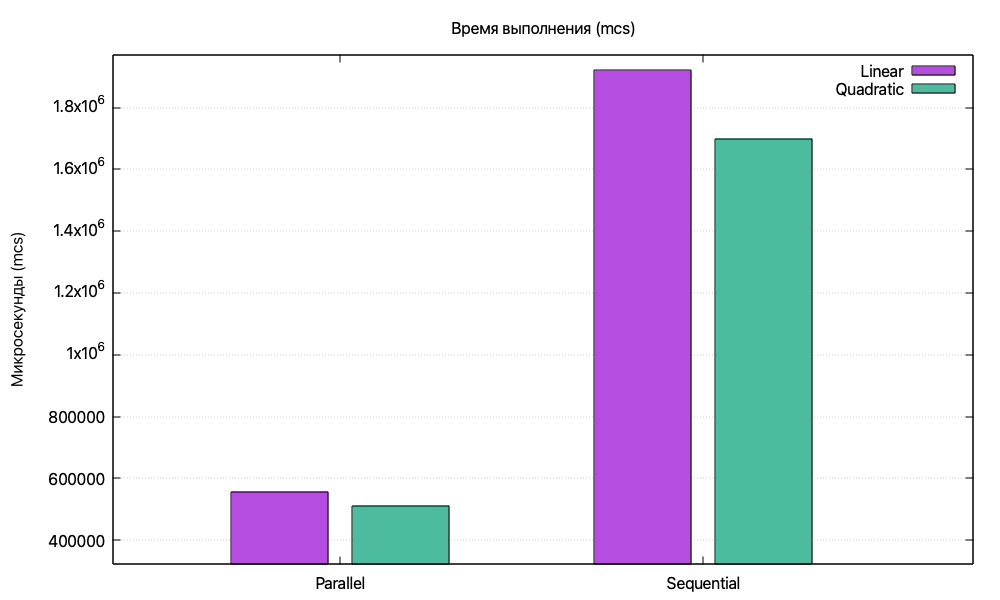
\includegraphics[width=0.9\textwidth]{img/four_dimensional_buildtype_basis.png}
    \caption{Сравнение всех сочетаний \texttt{BuildType} и \texttt{BasisType} на 4-мерной функции}
    \label{fig:four_dimensional_buildtype_basis_placeholder}
\end{figure}

\subsection{Сравнение Go- и C++-реализаций библиотеки}

Сопоставление двух реализаций усиливает инженерную ценность работы и позволяет говорить не только о корректности алгоритма, но и о свойствах различных способов его программного воплощения.

\subsubsection{Сравнение последовательных реализаций}

В последовательном режиме C++-реализация в большинстве сценариев показывает более низкое время построения, чем Go-реализация. Например, для бенчмарка масштабирования по размерности и области в 1D при масштабе $\pi$ получено 11698 нс против 18862 нс в Go. В 2D при масштабе $\pi$ --- 32706 нс против 49017 нс, а в 3D при масштабе $\pi$ --- 411503 нс против 674239 нс. Особенно показательно сравнение базисов: в C++ последовательной версии времена составляют 557459 нс против 293392 нс при $\varepsilon = 0.01$, 648720 нс против 305538 нс при $\varepsilon = 0.005$ и 1781085 нс против 638925 нс при $\varepsilon = 0.001$. Тем самым и в C++ квадратичный базис оказывается существенно выгоднее линейного на сложной тестовой функции.

Такой результат ожидаем. C++-версия использует более низкоуровневую модель исполнения и, вероятно, эффективнее работает с временными объектами и размещением данных в памяти. Поэтому в чисто последовательном режиме C++ закономерно оказывается быстрее.

\subsubsection{Сравнение параллельных реализаций}

Наиболее интересная часть сопоставления связана с параллельным режимом. В бенчмарке \texttt{ParallelVsSequentialBuild} C++ показывает очень близкие результаты для всех четырёх комбинаций: 4451 нс и 4493 нс для последовательных режимов, 4735 нс и 4196 нс для параллельных. Для Go на той же группе сценариев получены 7377917 и 2867911 нс для последовательных режимов, а также 5495296 и 2324588 нс для параллельных.

Следовательно, сравнение остаётся содержательным: в Go параллельный режим действительно даёт ускорение на нетривиальной двумерной функции. Это хорошо согласуется с назначением параллельной архитектуры и показывает, что её эффект проявляется именно там, где сетка перестаёт быть слишком простой.

При этом качественное замечание о модели исполнения сохраняется. В Go конкурентный код поддерживается встроенным scheduler, который эффективно управляет большим числом лёгких goroutine. В C++ использовался \texttt{std::async} с флагом \texttt{async}. Поэтому важно подчеркнуть не абсолютное превосходство одной платформы над другой, а различие в моделях конкурентного исполнения и в том, как они ведут себя на задачах разного масштаба.

\subsubsection{Сравнение режимов работы с дифференциальными уравнениями}

Для C++-версии выводы по двум подходам к работе с диффурами качественно совпадают с Go. В последовательном режиме итеративный подход через последовательные шаги устойчиво быстрее режима с параметром $t$ как дополнительной размерностью: 4372 нс против 22867 нс при $t_{max}=2$, 10027 нс против 46823 нс при $t_{max}=5$, 18543 нс против 66037 нс при $t_{max}=10$, 37723 нс против 75921 нс при $t_{max}=20$.

В Go получены 16384 нс против 103748 нс при $t_{max}=2$, 41559 нс против 196721 нс при $t_{max}=5$, 83561 нс против 280524 нс при $t_{max}=10$ и 169502 нс против 332080 нс при $t_{max}=20$. Следовательно, обе реализации дают одинаковый качественный вывод: в рассматриваемой постановке итеративный подход через последовательное применение одношагового оператора предпочтительнее, чем включение времени как отдельной координаты пространства аргументов.

\subsubsection{Сравнение ограничения числа узлов}

В обеих реализациях ограничение числа узлов демонстрирует одинаковый качественный эффект: чем меньше лимит, тем ниже время построения. В C++ последовательной версии без лимита получено 1932286 нс, а при лимите 200 --- 552059 нс. В параллельной версии --- 1935248 нс и 557735 нс соответственно. В Go получено 4833921 нс без ограничения и 972821 нс при лимите 200. Для лимитов 500 и 1000 получены 2160798 и 3104964 нс/оп.

Этот результат важен тем, что он носит платформенно-независимый характер. Механизм ограничения числа узлов работает как содержательное средство управления затратами и в Go, и в C++. Это подчёркивает, что его роль определяется не особенностями языка реализации, а самой архитектурой алгоритма.

% TODO_IMG: отдельный график для parallel-режима. Лучше сделать grouped bar chart по нескольким сценариям, потому что разница между Go и C++ в параллельном режиме может отличаться для малых и более тяжёлых задач. Можно отдельно сравнить small-case benchmark, diffur-режимы и 4-мерную функцию.
\begin{figure}[H]
    \centering
    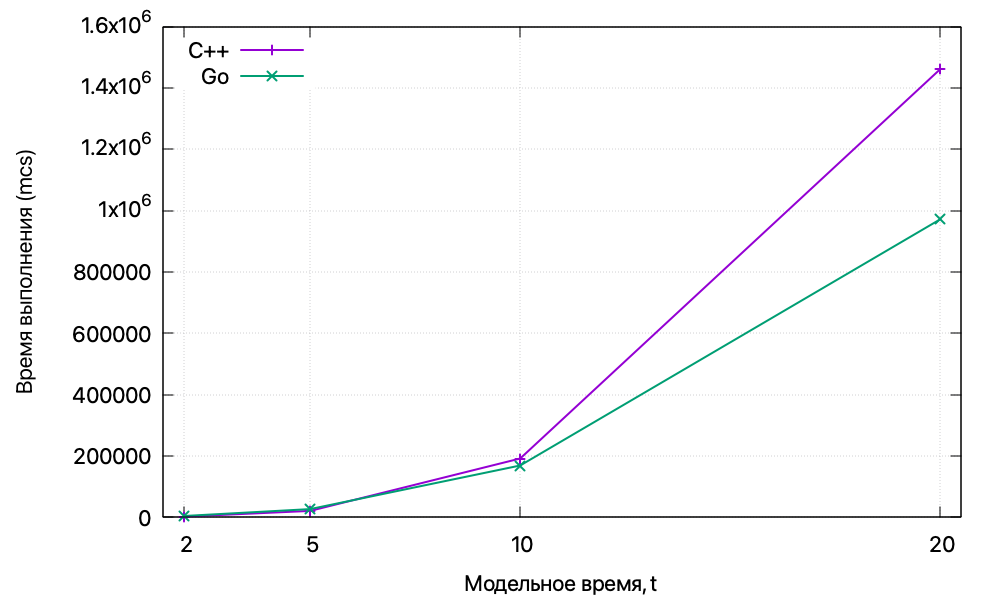
\includegraphics[width=0.9\textwidth]{img/go_vs_cpp.png}
    \caption{Сравнение Go- и C++-реализаций на примере итеративного решения дифференциального уравнения}
    \label{fig:go_vs_cpp_placeholder}
\end{figure}

\subsection{Преимущества разработанного решения}

На основе архитектуры проекта и экспериментальной программы можно выделить следующие преимущества разработанного решения:
\begin{enumerate}
    \item модуль \texttt{compute} объединяет математическую компактность и практическую гибкость;
    \item поддержка двух базисов позволяет исследовать баланс между локальной стоимостью и качеством аппроксимации;
    \item механизм anchor points расширяет базовый метод и устраняет важный класс ошибок адаптивного критерия;
    \item параметр ограничения числа узлов даёт эффективный способ контролировать ресурсы;
    \item поддержка двух режимов работы с дифференциальными уравнениями делает систему более универсальной;
    \item экспериментальная программа позволяет анализировать поведение алгоритма в нескольких содержательных режимах, а не только на одном частном тесте;
    \item сравнение Go- и C++-версий усиливает инженерную ценность работы и позволяет говорить не только о корректности алгоритма, но и о свойствах различных способов его реализации.
\end{enumerate}

\subsection{Ограничения текущей реализации}

Несмотря на полученные результаты, текущая версия системы имеет и ряд ограничений.

\begin{enumerate}
    \item Клиентская визуализация ориентирована прежде всего на двумерные задачи и не предоставляет развитых средств анализа для более высоких размерностей.
    \item Выбор anchor points производится вручную; автоматизированной стратегии их генерации пока не реализовано.
    \item Для полного количественного анализа качества интерполяции требуется дальнейшее расширение набора тестовых функций и метрик ошибки.
    \item В проекте пока отсутствует встроенная автоматическая генерация графиков по результатам бенчмарков, поэтому соответствующие иллюстрации подготавливаются отдельно.
    \item Этап вычисления значения по готовой сетке требует дополнительной оптимизации из-за высокой стоимости рекурсивного обхода и большого числа повторных вычислений.
    \item Для более строгого межъязыкового сопоставления в будущем полезно автоматизировать единый контур запуска и экспорта результатов Go- и C++-бенчмарков в один формат.
\end{enumerate}

\subsection{Иллюстрации двумерных функций, полученные во Flutter-клиенте}

Для качественной оценки поведения алгоритма важно анализировать не только численные бенчмарки, но и визуальную структуру построенных сеток. Flutter-клиент позволяет наглядно увидеть отображение, задаваемое функцией и построенное по тем же данным, что используются в вычислительном модуле.

На рисунке \ref{fig:flutter_simple} показана визуализация функции
\begin{equation}
    u = x, \qquad v = y\left(\sin(2.5x) + 0.35\cos(6y) + 0.2\sin(5x + 0.4) - 0.15\cos(9y - 0.2)\right)
\end{equation}
на области
\begin{equation}
    x \in [0, 4], \qquad y \in [0, 2]
\end{equation}
при
\begin{equation}
    \varepsilon = 0.001.
\end{equation}
Такой пример удобен тем, что не содержит смешанных членов вида $\sin(xy)$, но при этом создаёт более содержательную структуру двумерной сетки. Это позволяет визуально увидеть, как адаптивная сетка концентрирует узлы в более сложных областях, не перегружая всю область равномерным дискретизационным шаблоном.

% TODO_IMG: использовать скриншот функции u=x, v=y*(sin(2.5x)+0.35cos(6y)+0.2sin(5x+0.4)-0.15cos(9y-0.2)) на области x in [0,4], y in [0,2] при epsilon=0.001. Желательно, чтобы на изображении были дополнительно отмечены точки-узлы сетки, чтобы была видна их плотность в разных частях области.
\begin{figure}[H]
    \centering
    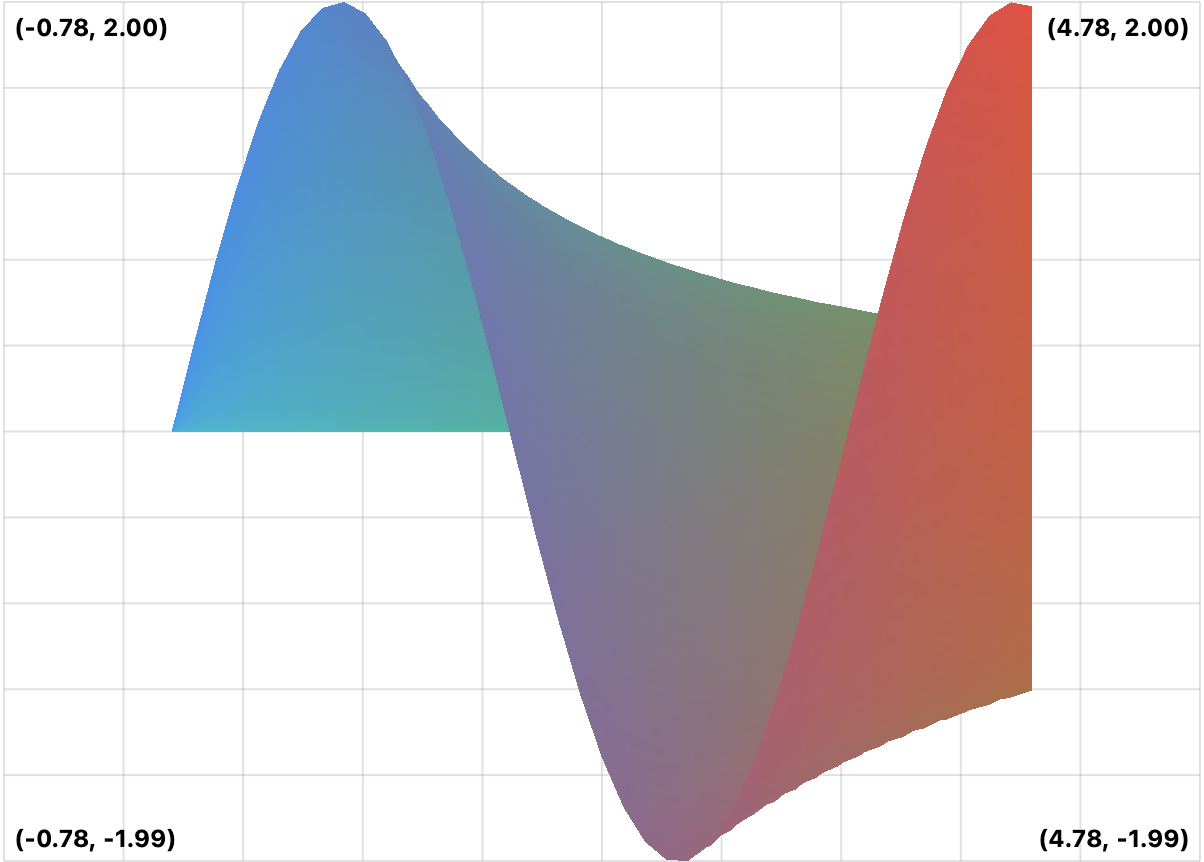
\includegraphics[width=0.9\textwidth]{img/flutter_simple.png}
    \caption{Визуализация функции $u=x$, $v=y(\sin(2.5x)+0.35\cos(6y)+0.2\sin(5x+0.4)-0.15\cos(9y-0.2))$ во Flutter-клиенте}
    \label{fig:flutter_simple}
\end{figure}

На рисунке \ref{fig:flutter_diffur} представлен пример визуализации динамической задачи, задаваемой системой
\begin{equation}
    \frac{dx}{dt} = 0, \qquad \frac{dy}{dt} = \sin(x)\,y + t
\end{equation}
при начальных условиях
\begin{equation}
    x \in [-2, 5], \qquad y \in [0, 1]
\end{equation}
и при
\begin{equation}
    \varepsilon = 0.001.
\end{equation}
Этот пример особенно полезен для демонстрации того, что адаптивная интерполяция применима не только к аналитическим функциям, но и к отображениям, возникающим из численного интегрирования дифференциальных уравнений. На изображении можно увидеть, как локальная сложность динамики приводит к неоднородному распределению узлов.

% TODO_IMG: использовать скриншот системы dx/dt=0, dy/dt=sin(x)*y+t на области x in [-2,5], y in [0,1] при epsilon=0.001. Желательно также показать точки-узлы, чтобы была заметна адаптивная плотность сетки в областях более сложной динамики.
\begin{figure}[H]
    \centering
    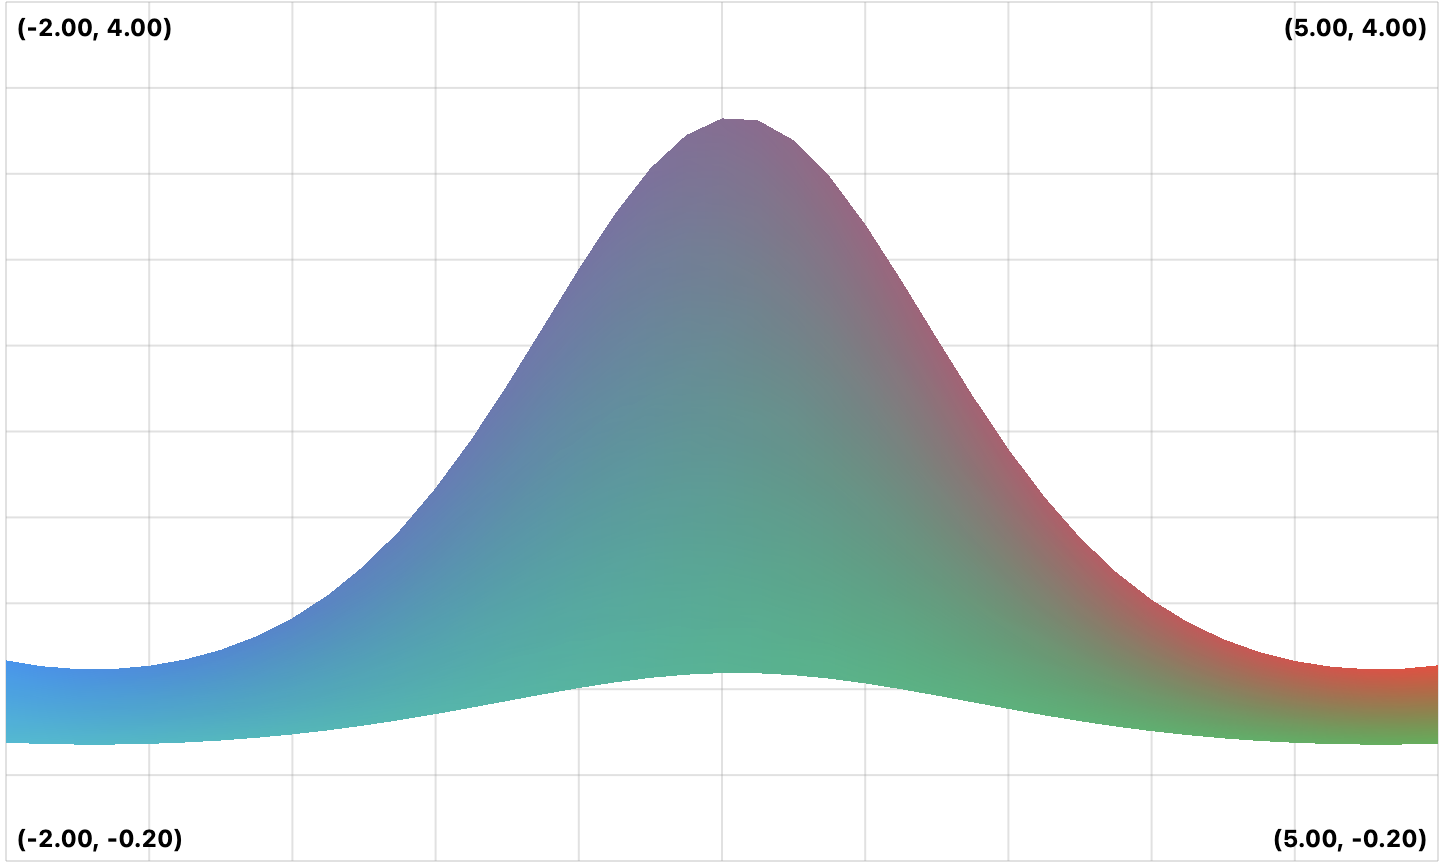
\includegraphics[width=0.9\textwidth]{img/flutter_differential.png}
    \caption{Визуализация дифференциального уравнения во Flutter-клиенте}
    \label{fig:flutter_diffur}
\end{figure}

\subsection{Перспективы дальнейшего развития}

Дальнейшее развитие проекта может идти по нескольким направлениям:
\begin{enumerate}
    \item автоматизация выбора anchor points на основе анализа локальной структуры ошибки;
    \item расширение визуализации на многомерные случаи;
    \item добавление встроенного контура сохранения результатов бенчмарков и генерации графиков;
    \item расширение библиотеки тестовых сценариев для количественного исследования норм ошибки;
    \item оптимизация рекурсивного этапа вычисления значения по готовой сетке;
    \item исследование комбинированных стратегий выбора базиса и ограничения числа узлов в зависимости от характера функции;
    \item разработка единого автоматизированного режима сравнения Go- и C++-версий библиотеки.
\end{enumerate}

\subsection*{Выводы по главе}
\addcontentsline{toc}{subsection}{Выводы по главе}

В четвёртой главе был проведён развёрнутый анализ результатов дипломной работы с акцентом на экспериментальную программу и производительность вычислительного модуля \texttt{compute}. Показано, что усложнение двумерных тестовых функций делает бенчмарки значительно более показательными: главная двумерная сетка перестаёт вырождаться в почти тривиальную структуру, а различия между режимами исполнения и типами базиса начинают отчётливо проявляться на уровне времени построения. Измерения для Go-реализации подтвердили устойчивое преимущество квадратичного базиса, заметный выигрыш параллельного режима на нетривиальных двумерных функциях, высокую эффективность итеративного подхода при работе с дифференциальными уравнениями и практическую значимость ограничения числа узлов как средства управления затратами. Дополнительное сопоставление Go- и C++-реализаций показало, что C++-версия быстрее в абсолютных значениях на значительной части рассмотренных тестов, однако обе реализации демонстрируют одинаковые качественные закономерности. В совокупности полученные результаты подтверждают достижение цели дипломной работы и создают основу для дальнейшего развития проекта.
